% MMM Project - Marketing Mix Modeling Report
\documentclass[11pt,a4paper]{article}
\usepackage[utf8]{inputenc}
\usepackage[T1]{fontenc}
\usepackage[french]{babel}
\usepackage{graphicx}
\usepackage[hidelinks]{hyperref}
\usepackage{geometry}
\usepackage{booktabs}
\usepackage{caption}
\usepackage{float}
\geometry{margin=2.5cm}
\graphicspath{{Assets/}}

\title{Rapport du Projet MMM - Marketing Mix Modeling}
\author{Equipe MMM}
\date{\today}

\begin{document}

\maketitle
\begin{abstract}
Ce rapport présente la conception et l'implémentation d'un projet de Marketing Mix Modeling (MMM) intégrant un pipeline ETL, une modélisation MMA de base et un tableau de bord Streamlit pour l'analyse des performances marketing.
\end{abstract}

\section{Introduction}
Le projet vise à fournir une solution complète pour mesurer l'efficacité des canaux marketing, estimer les contributions des investissements médias et proposer des scénarios budgétaires.
La solution combine :
\begin{itemize}
  \item une préparation de données structurée depuis des sources brutes,
  \item un jeu de données transformé prêt pour la modélisation,
  \item une interface de visualisation interactive,
  \item un modèle de référence permettant de générer des métriques et des attributions.
\end{itemize}

\section{Architecture du projet}
Le projet est organisé autour d'un pipeline de données, d'un module de modélisation et d'un tableau de bord.
Figure~\ref{fig:architecture} décrit l'architecture globale.

\begin{figure}[H]
  \centering
  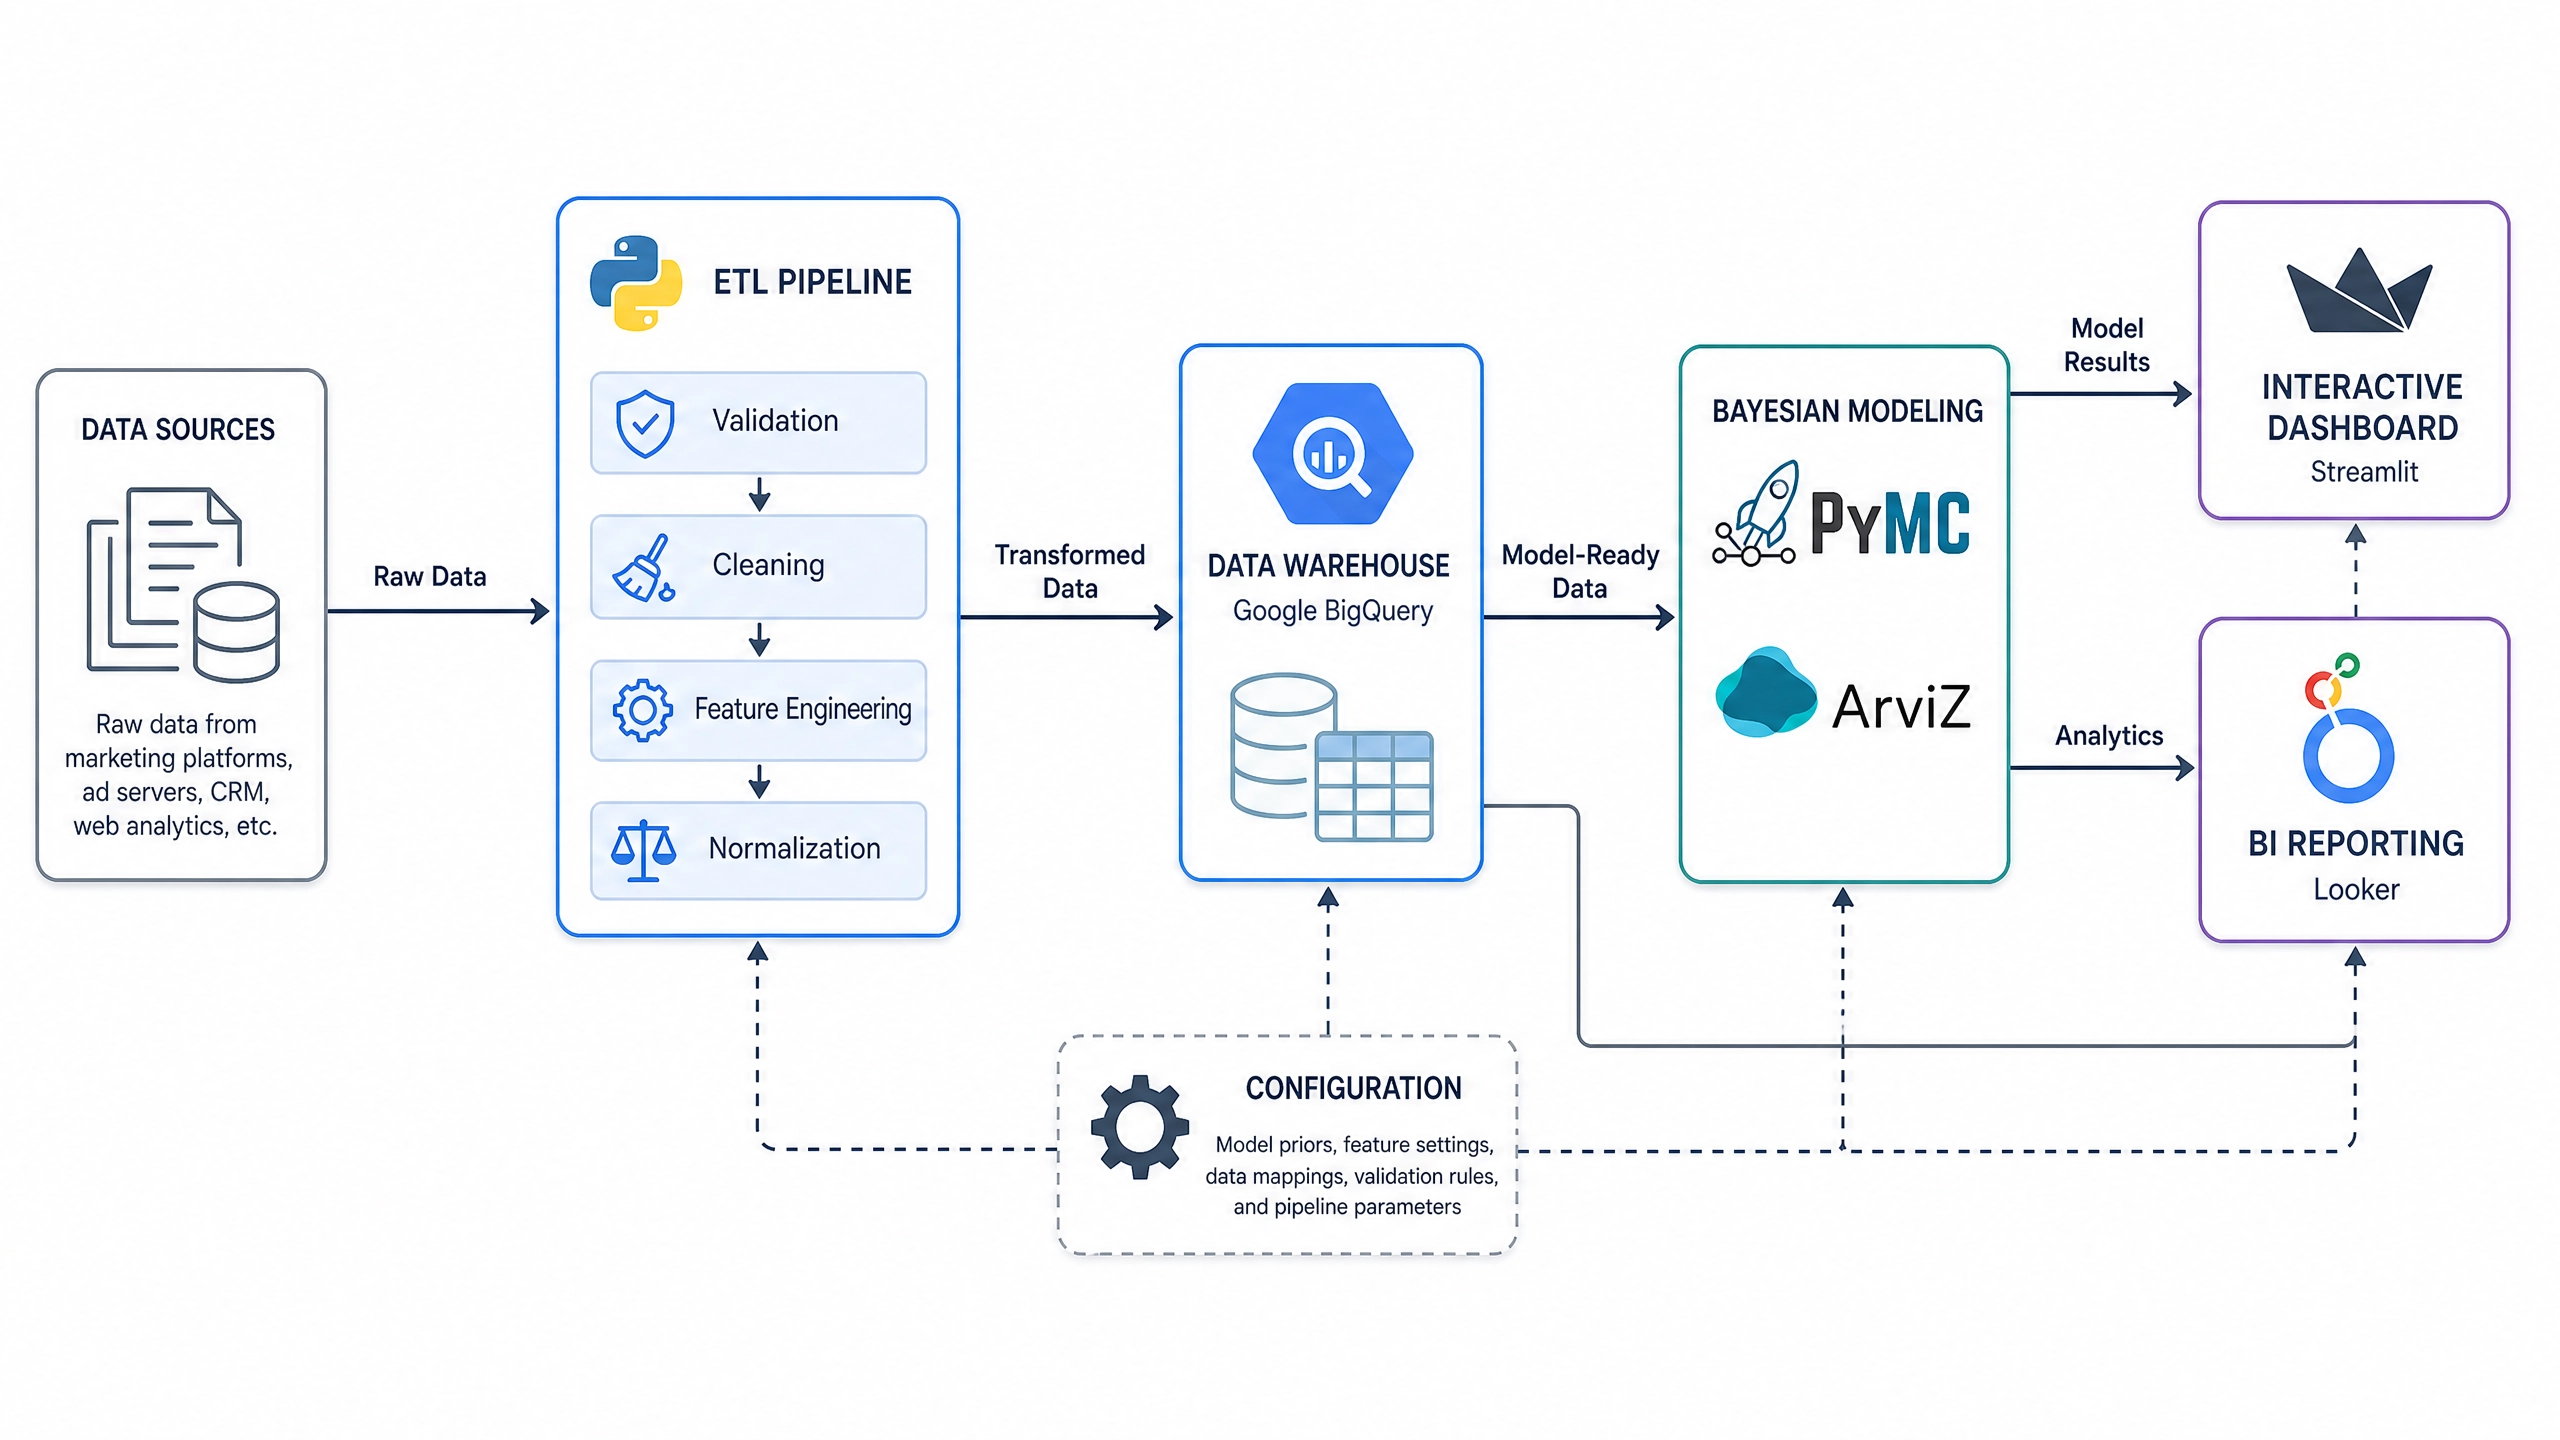
\includegraphics[width=0.95\textwidth]{architecture_mmm.png}
  \caption{Architecture du pipeline MMM}
  \label{fig:architecture}
\end{figure}

\section{Pipeline ETL}
Le pipeline ETL lit les données brutes depuis \texttt{data/raw/}, applique des nettoyages, enrichit les observations avec des événements et des variables temporelles, puis produit le jeu de données final \texttt{data/processed/mmm_ready.csv}.
Les composants principaux du pipeline incluent :
\begin{itemize}
  \item \texttt{etl/clean.py} pour le nettoyage et la normalisation initiale,
  \item \texttt{etl/event_enrichment.py} pour les features basées sur calendrier et événements,
  \item \texttt{etl/feature_engineering.py} pour le calcul d'adstock, de saturations et d'interactions,
  \item \texttt{etl/load_bigquery.py} pour le chargement optionnel dans BigQuery.
\end{itemize}

\section{Préparation des features}
La préparation des features contient des transformations marketing essentielles :
\begin{itemize}
  \item adstock pour capturer l'effet retardé des dépenses,
  \item saturations pour modéliser les rendements décroissants,
  \item interactions entre canaux pour capturer les synergies marketing.
\end{itemize}

\section{Modèle MMM}
Une implémentation de modèle de référence est disponible dans \texttt{models/mmm_model.py}.
Ce modèle utilise :
\begin{itemize}
  \item une régression Ridge avec normalisation StandardScaler,
  \item des features marketing adstockées telles que celles se terminant par \texttt{\_SPEND\_ADSTOCK\_SAT},
  \item des variables de contrôle temporelles (jour de la semaine, saisonnalité, tendance).
\end{itemize}

Les principales étapes du modèle sont :
\begin{enumerate}
  \item sélection de la cible de revenue (`FIRST_PURCHASES_ORIGINAL_PRICE`, `REVENUE`, `FIRST_PURCHASES`),
  \item extraction des features de canal et des variables de contrôle,
  \item entraînement du modèle et évaluations de performance (R2, MSE),
  \item estimation des contributions par canal,
  \item simulation de scénarios budgétaires.
\end{enumerate}

\section{Tableau de bord Streamlit}
Le tableau de bord principal est \texttt{dashboard/app.py} et fournit des pages dédiées aux objectifs suivants :
\begin{itemize}
  \item indicateurs clés et tendances,
  \item analyse des canaux,
  \item scénarios budgétaires et simulations,
  \item attribution multi-touch,
  \item intégration Looker.
\end{itemize}

\begin{figure}[H]
  \centering
  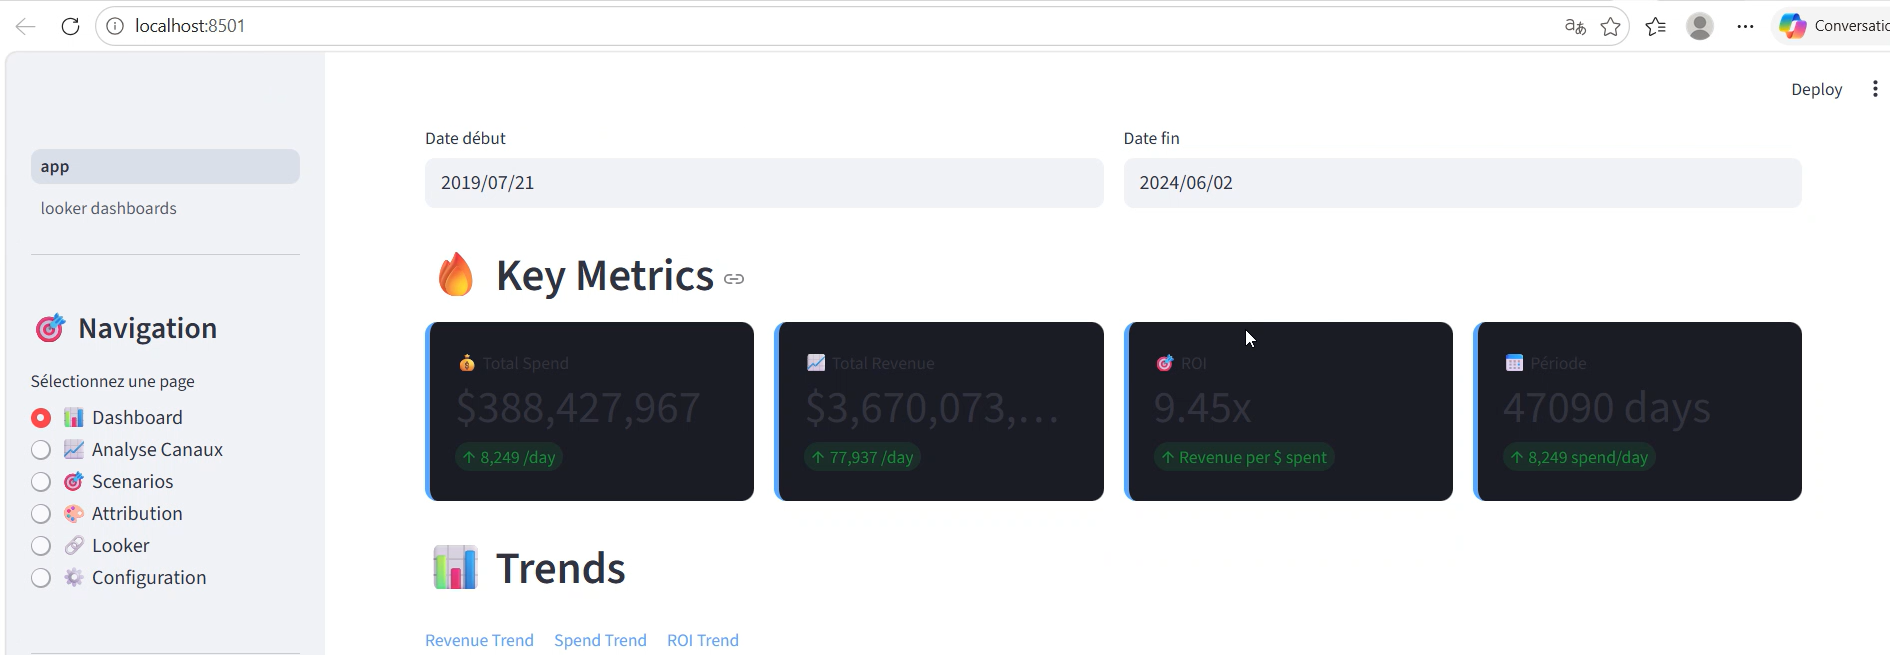
\includegraphics[width=0.95\textwidth]{Interface_dashboard.png}
  \caption{Capture d'écran du dashboard Streamlit}
  \label{fig:dashboard}
\end{figure}

\section{Visualisation et reporting}
Le projet contient des captures d'écran illustrant les analyses clés.

\begin{figure}[H]
  \centering
  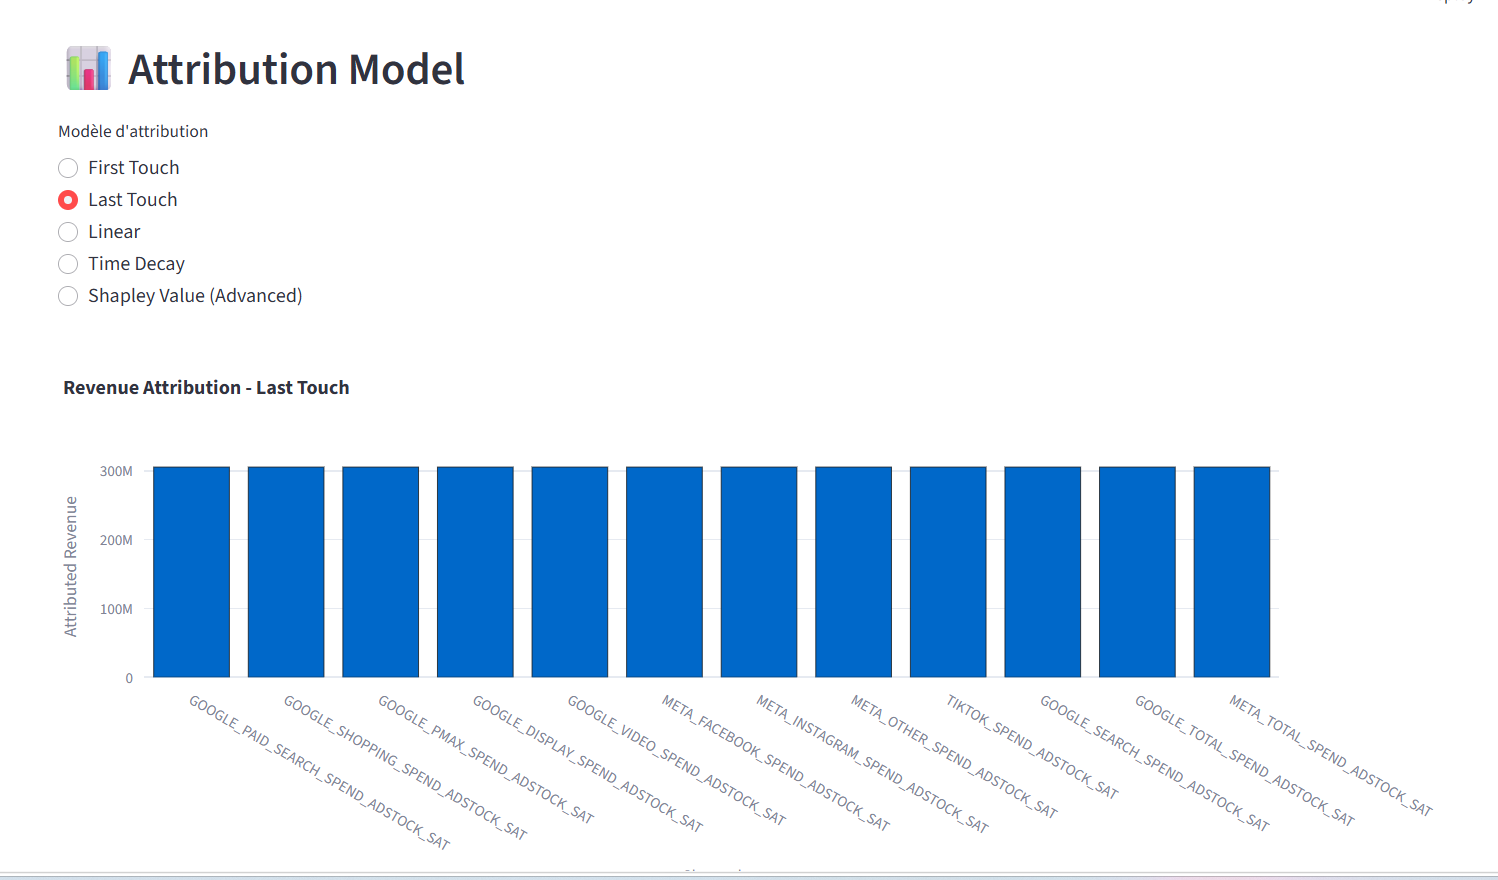
\includegraphics[width=0.8\textwidth]{Attribution_multi_touch.png}
  \caption{Analyse d'attribution multi-touch}
\end{figure}

\begin{figure}[H]
  \centering
  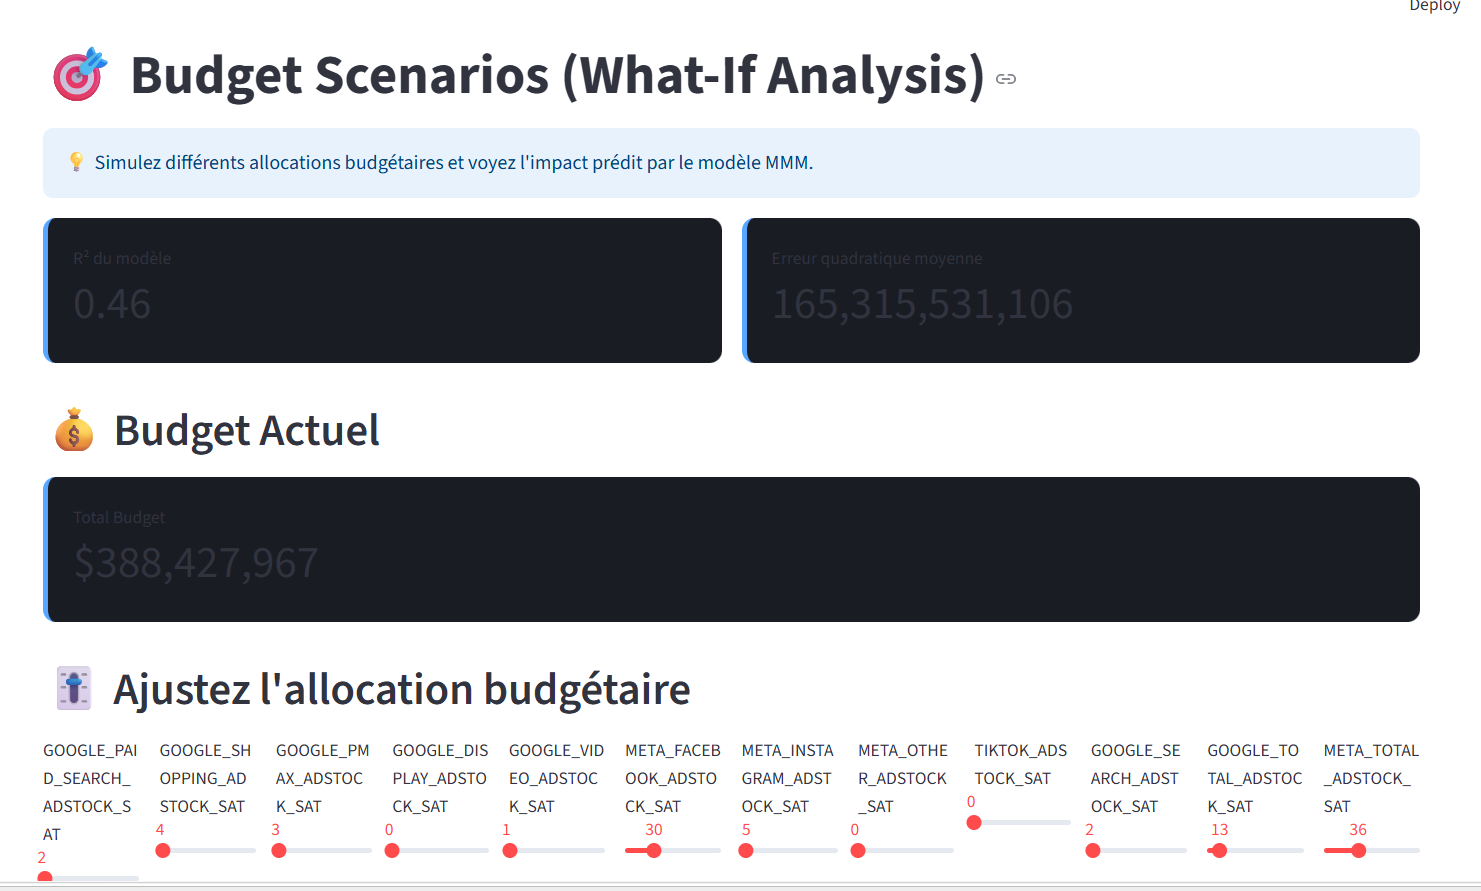
\includegraphics[width=0.8\textwidth]{Budget_Scenarios_What_if.png}
  \caption{Scénarios budgétaires et simulations}
\end{figure}

\begin{figure}[H]
  \centering
  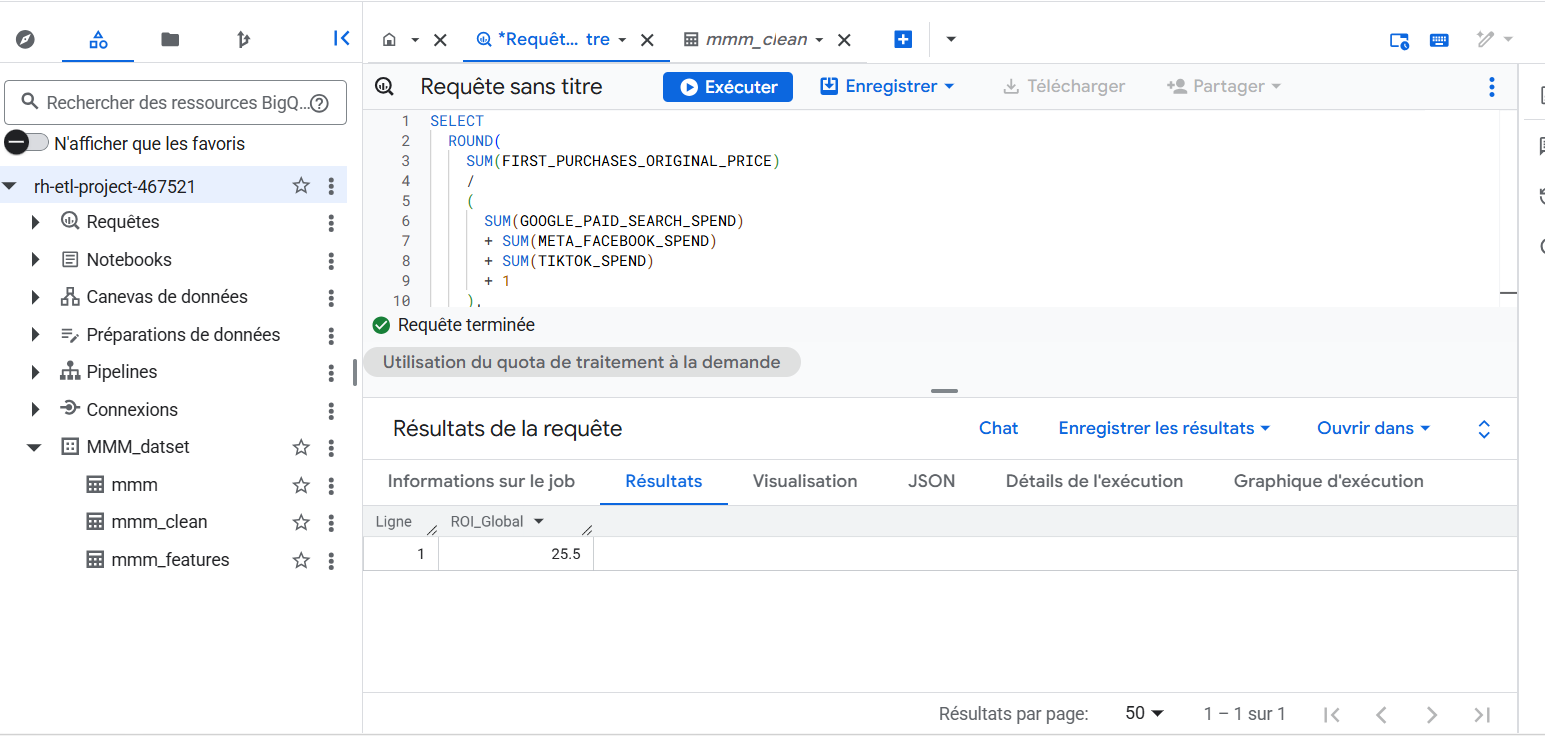
\includegraphics[width=0.8\textwidth]{ROI_Global.png}
  \caption{Vue d'ensemble du ROI global}
\end{figure}

\section{Résultats et discussion}
Le modèle de référence fournit une première estimation des contributions des canaux sur le revenu et sert de base pour les futurs développements.
Les visualisations du dashboard permettent de comparer les dépenses et la rentabilité par canal, ainsi que d'analyser des scénarios de réallocation budgétaire.

\section{Perspectives}
Les extensions recommandées comprennent :
\begin{itemize}
  \item migration vers une modélisation Bayésienne complète avec \texttt{pymc} et \texttt{arviz},
  \item validation plus robuste par cross-validation temporelle,
  \item amélioration des interactions et des termes non-linéaires,
  \item déploiement Cloud de l'application Streamlit.
\end{itemize}

\section{Conclusion}
Ce projet fournit un cadre opérationnel pour l'analyse MMM et la production de rapports marketing.
La solution est déjà utilisable localement avec le tableau de bord Streamlit et le jeu de données transformé, tout en restant extensible vers des modèles plus avancés.

\end{document}
